\documentclass[10pt]{beamer}

%\usetheme{ENSLyon}

\usetheme{AnnArbor}

\title[CNMAC 2021]{\large \textsc{Geometria de Distâncias e Álgebras Geométricas \\ Aplicadas a Conformação Molecular}}
\author[G. Philippi]{{Guilherme Philippi\vspace{-0.3cm}}}
\institute[]{Departamento de Matemática\\ Universidade Federal de Santa Catarina, Blumenau \\ \vspace{0.2cm} \normalsize Orientado por Felipe Fidalgo \vspace{-0.2cm}}
\date[23 Novembro, 2021]{ {\small 4$^\text{o}$ Seminário de Iniciação Científica} \\ {\scriptsize UFSC Campus Blumenau\\ 23 de novembro de 2021}}
\setbeamersize{text margin left=5mm}
\setbeamersize{text margin right=5mm}

\setbeamertemplate{navigation symbols}{}
%\usecolortheme{ENSLyon_greener}
\usecolortheme{whale}

\setbeamercolor{frametitle}{bg=gray}
\setbeamertemplate{bibliography item}{\insertbiblabel}

%PACKAGES -------------------------
\usepackage{etex}
\usepackage[utf8]{inputenc}
\usepackage[brazilian]{babel}
\usepackage{enumerate}
\usepackage{amsmath}
\usepackage{amssymb}
\usepackage{amsthm}
\usepackage{amscd}
\usepackage{amsfonts}
\usepackage{multicol}
\usepackage{multirow}
\usepackage{array}
\usepackage{color}
\usepackage{graphicx}
\usepackage{tikz}
\usepackage{tikz-qtree}
\usepackage{wrapfig}
\usepackage{3dplot}
\usepackage{pgf}
\usepackage{makecell}
\usepackage{xltabular}
\usepackage{multirow}
\usepackage{siunitx}
\usepackage{tkz-euclide}
\usepackage{algorithmic}
\usepackage{algorithm}
\usepackage{xparse}
\usepackage{subfigure}

%LIBRARIES-TIKZ ------------------------------------------

\usetikzlibrary{shadows,trees}
\usetikzlibrary{decorations.pathmorphing}
\usetikzlibrary{decorations.markings}
\usetikzlibrary{positioning}
\usetikzlibrary{chains,matrix,scopes}
\usetikzlibrary{arrows}

%DEFINITIONS ----------------------------------------------------

\def\centerarc[#1](#2)(#3:#4:#5)% Syntax: [draw options] (center) (initial angle:final angle:radius)
{ \draw[#1] ($(#2)+({#5*cos(#3)},{#5*sin(#3)})$) arc(#3:#4:#5); }
\def\xx{\mathbf{x}}
\def\ii{\mathbf{i}}
\def\jj{\mathbf{j}}
\def\kk{\mathbf{k}}
\def\tt{\mathbf{t}}
\def\ee{\mathbf{e}}
\def\qq{\mathbf{q}}
\def\pp{\mathbf{p}}
\def\vv{\mathbf{v}}
\def\rr{\mathbf{r}}
\def\vzero{\mathbf{0}}
\def\qset{\mathbb{H}}
\def\xx{\mathbf{x}}


\AtBeginSection[]
{
	\begin{frame}<beamer>
		\frametitle{Inicio da seção \thesection}
		\tableofcontents[currentsection]
	\end{frame}
}


%NEW THEOREMS ------------------------------------------

\theoremstyle{plain}
\newtheorem{teorema}{Teorema}[section]
\newtheorem{lema}{Lema}[section]
\newtheorem{proposicao}{Proposição}[section]
\newtheorem{corolario}{Corolário}[section]

\theoremstyle{definition}
\newtheorem{definicao}{Definição}[section]
\newtheorem{observacao}{Observação}[section]
\newtheorem{exemplo}{Exemplo}[section]

\newenvironment{solucao}
{\renewcommand\qedsymbol{$\triangle$}\begin{proof}[Solução]}{\end{proof}}



\begin{document}
	
	%FACE
	\begin{frame}
		
		\titlepage
		
		\vspace{-0.7cm}
		\begin{flushleft}
			
\includegraphics[scale=0.16]{logo.png}
		\end{flushleft}
		
		\vspace{-2.3cm}
		\begin{flushright}
			
\includegraphics[scale=0.024]{logo_ufsc.png}
		\end{flushright}
	\end{frame}
	
	%Indice
	\begin{frame}
		\tableofcontents 
	\end{frame}
	
	\section{Motivação}
	
	\begin{frame}
		\frametitle{\normalsize Worldwide PDB } 
		{
			\small
			
			\begin{center}
				
\includegraphics[width=0.4\linewidth]{wwpdb-logo.png}	
			\end{center}
			
			Todas as informações sobre a estrutura 3D de proteínas são concentradas no repositório Protein Data Bank (PDB) \cite{PDB}.
			
			\begin{center}
				\begin{minipage}{0.08\linewidth}
					\hspace{0.1cm}
				\end{minipage}	
				\begin{minipage}{0.4\linewidth}
					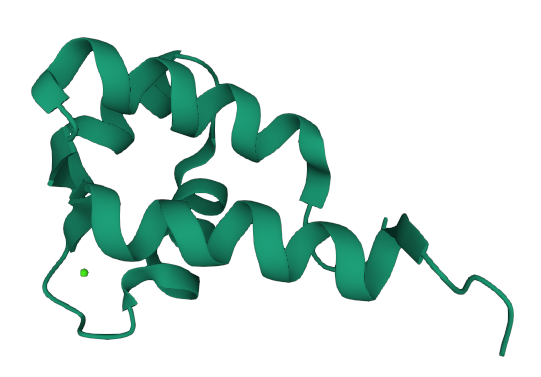
\includegraphics[width=0.8\linewidth]{prot2.png}
				\end{minipage}
				\begin{minipage}{0.08\linewidth}
					\hspace{0.5cm}
				\end{minipage}
				\begin{minipage}{0.4\linewidth}
					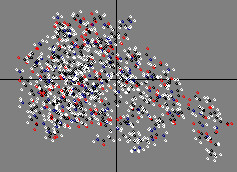
\includegraphics[width=0.7\linewidth]{prot.png}
				\end{minipage}
			\end{center}
		}	
	\end{frame}

	\begin{frame}
		\frametitle{\normalsize Motor muscular } 
		{
			\small
			
			\begin{center}
				\begin{minipage}{0.08\linewidth}
					\hspace{0.1cm}
				\end{minipage}	
				\begin{minipage}{0.3\linewidth}
					\centering Actina\\
					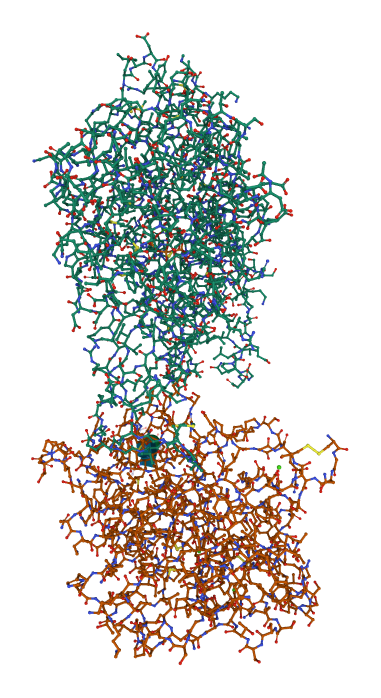
\includegraphics[width=1\linewidth]{1ATN.png}
				\end{minipage}
				\begin{minipage}{0.08\linewidth}
					\hspace{0.2cm}
				\end{minipage}
				\begin{minipage}{0.5\linewidth}
					\centering Miosina\\
					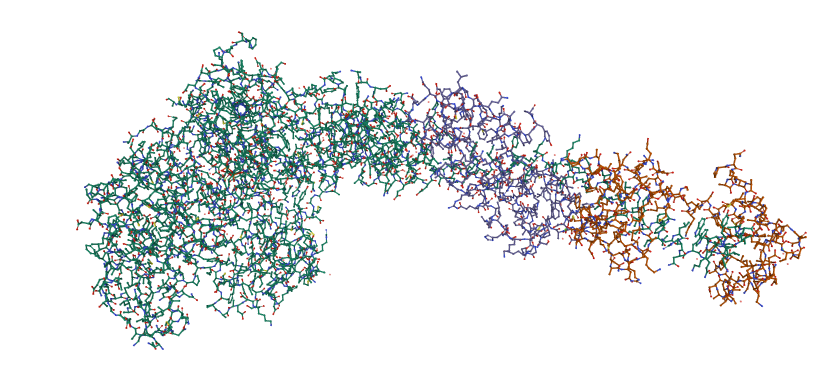
\includegraphics[width=1\linewidth]{1B7T.png}\\
					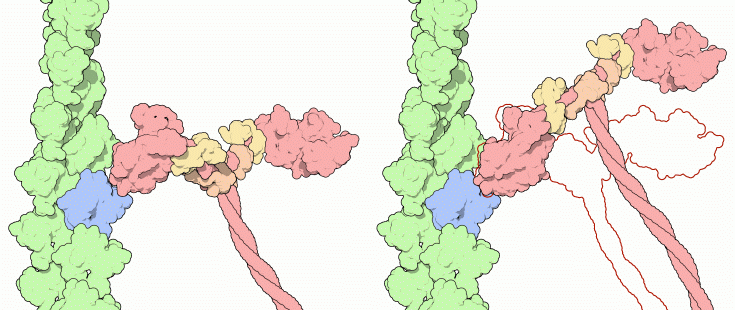
\includegraphics[width=1\linewidth]{powerstroke.png}
				\end{minipage}
			\end{center}
			
		}	
	\end{frame}

	\begin{frame}
		\frametitle{\normalsize Motor muscular } 
		{
			\small
			\begin{center}
				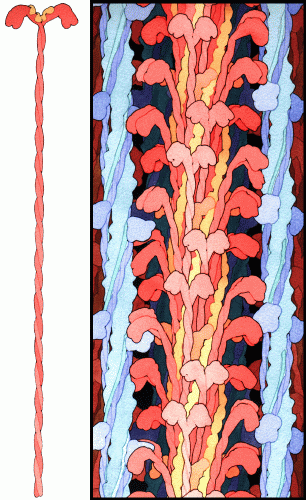
\includegraphics[width=0.4\linewidth]{myosin-painting.png}	
			\end{center}
			
		}	
	\end{frame}
	
	\section{Nosso problema}
	
	\begin{frame}
		\frametitle{\normalsize Geometria de Distâncias} 
		{
			\small
			\begin{definicao}[Distance Geometry Problem (DGP) \cite{carlileGDandAplications}]
				Dados um grafo simples, ponderado e conectado $G = (V, E, d)$ e um inteiro $K>0$, encontre uma realização $x: V \longrightarrow \mathbb{R}^K$ tal que:
				\begin{equation*}
					\forall \{u,v\} \in E, \hspace{0.5cm} \lVert x(u) - x(v) \rVert = d(\{u,v\}). \label{eq:DGP}
				\end{equation*}	
			\end{definicao}
			\begin{center}
				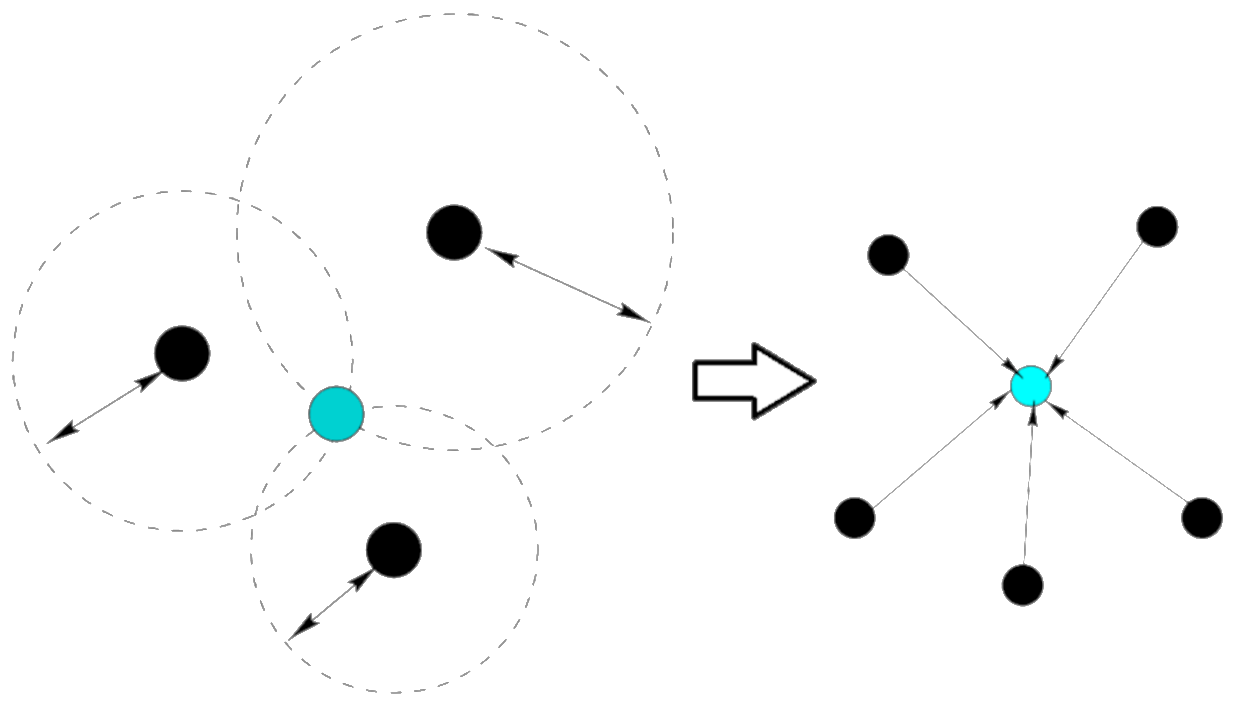
\includegraphics[width=0.5\linewidth]{dgp.png}
			\end{center}
		
			Chamamos $G$ de grafo DGP. Esse é um problema \textbf{NP}-completo para $K = 1$ e \textbf{NP}-difícil para $K>1$ \cite{Saxe:79}.
			}	
	\end{frame}

	\begin{frame}
		\frametitle{\normalsize Discretização do problema molecular} 
		{
			\small
			\begin{definicao}[Discretizable Molecular DGP (DMDGP) \cite{carlile:MinimalOrder}]
				Dado um grafo DGP e uma ordenação nos vértices $v_1,\dots,v_n$ tal que
				\begin{itemize}
					\item Existe uma realização válida para $v_1, v_2, v_3$ e
					\item Para todo $i \geq 4$, o conjunto $\{v_{i-3}, v_{i-2}, v_{i-1}, v_i\}$ é um clique com $$d_{i-3,i-2} + d_{i-2,i-1} > d_{i-3,i-1},$$
				\end{itemize}
				encontre uma realização $x: V \longrightarrow \mathbb{R}^3$ tal que 
				$$\forall \{u,v\} \in E, \hspace{0.5cm} \lVert x(u) - x(v) \rVert = d(\{u,v\}).$$
			\end{definicao}
			\begin{center}
				\begin{minipage}{0.8\linewidth}
					\hspace{0.05cm}
				\end{minipage}	
				\begin{minipage}{0.3\linewidth}
					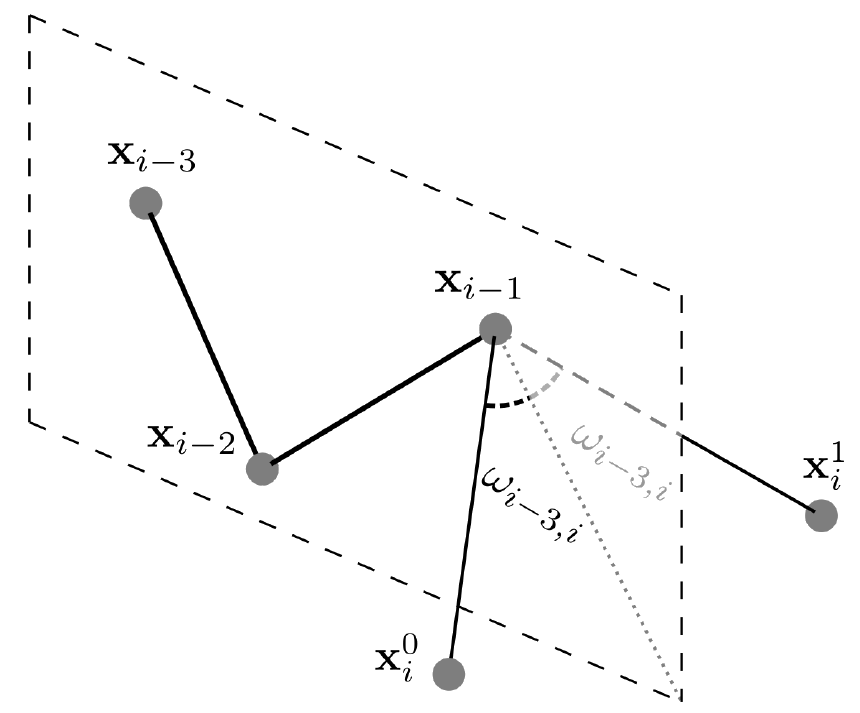
\includegraphics[width=0.95\linewidth]{dmdgp.png}
				\end{minipage}
				\begin{minipage}{0.2\linewidth}
					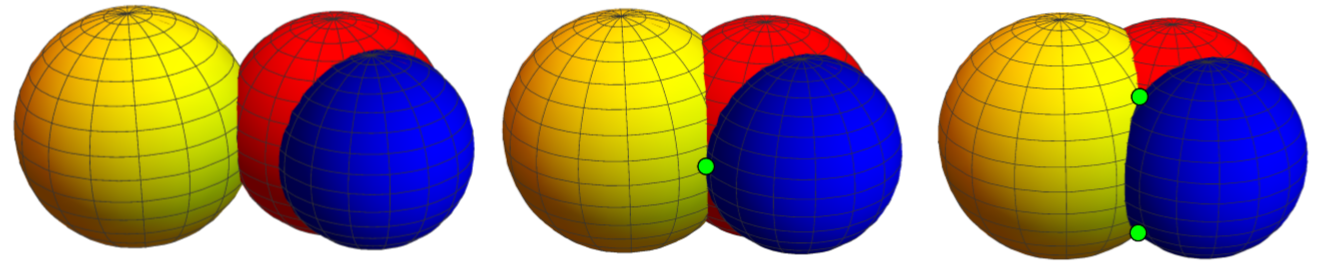
\includegraphics[width=1.2\linewidth]{esferas.png}
				\end{minipage}
				\begin{minipage}{0.08\linewidth}
					\hspace{0.2cm}
				\end{minipage}
				\begin{minipage}{0.2\linewidth}
					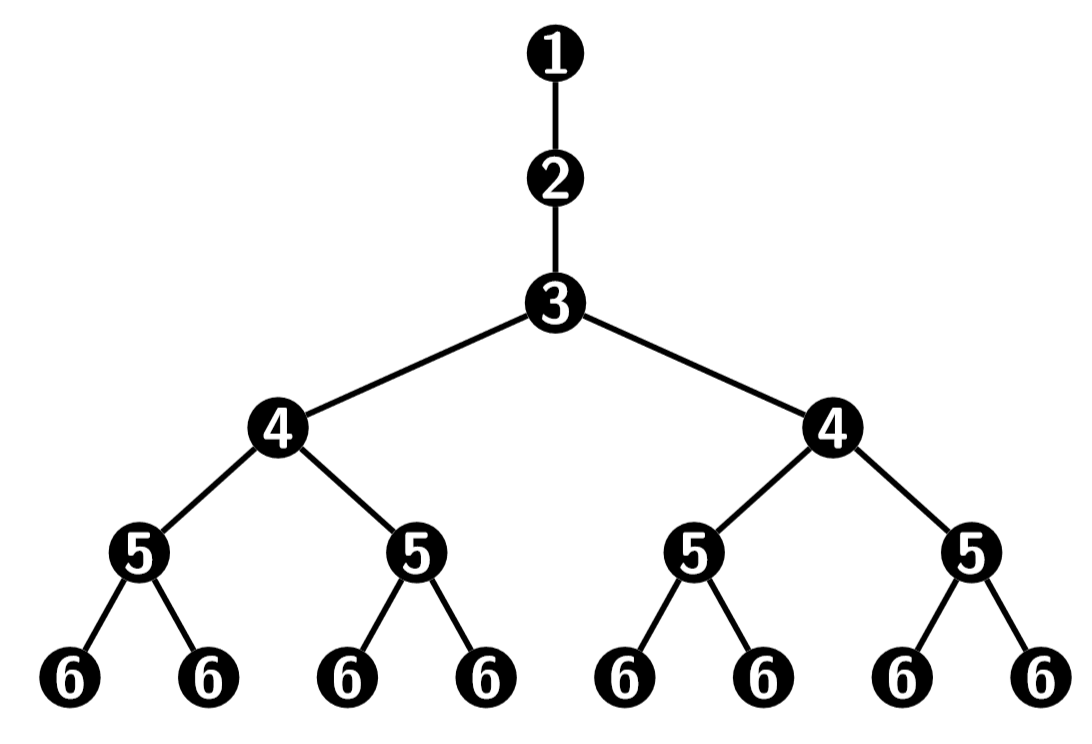
\includegraphics[width=1.4\linewidth]{ramificacoes.png}
				\end{minipage}
			\end{center}
		}	
	\end{frame}
	
	\begin{frame}
		\frametitle{\normalsize Algoritmo Branch-\&-Prune (BP)} 
		{
			\small
			\begin{center}
				É definido em três partes: Inicialização, branch e prune.
				\\
				\begin{center}
					\begin{minipage}{0.01\linewidth}
						\hspace{0.05cm}
					\end{minipage}	
					\begin{minipage}{0.42\linewidth}
						%\hspace{1.1cm}
						\includegraphics[width=1\linewidth]{inicializationgray-eps-converted-to.pdf}
					\end{minipage}
					\begin{minipage}{0.2\linewidth}
						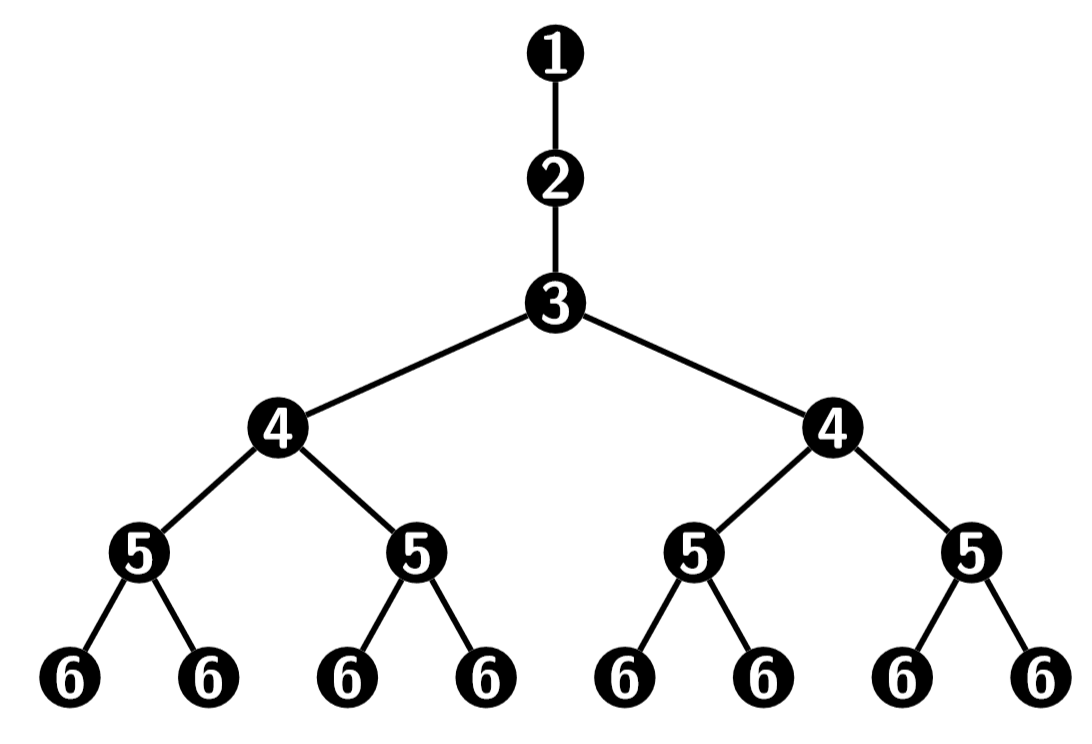
\includegraphics[width=1.5\linewidth]{ramificacoes.png}
					\end{minipage}
					\begin{minipage}{0.08\linewidth}
						\hspace{0.2cm}
					\end{minipage}
				\end{center}
			\end{center}
			
			
			
			\begin{center}
				\begin{minipage}{0.8\linewidth}
					\hspace{0.05cm}
				\end{minipage}	
				\begin{minipage}{0.3\linewidth}
					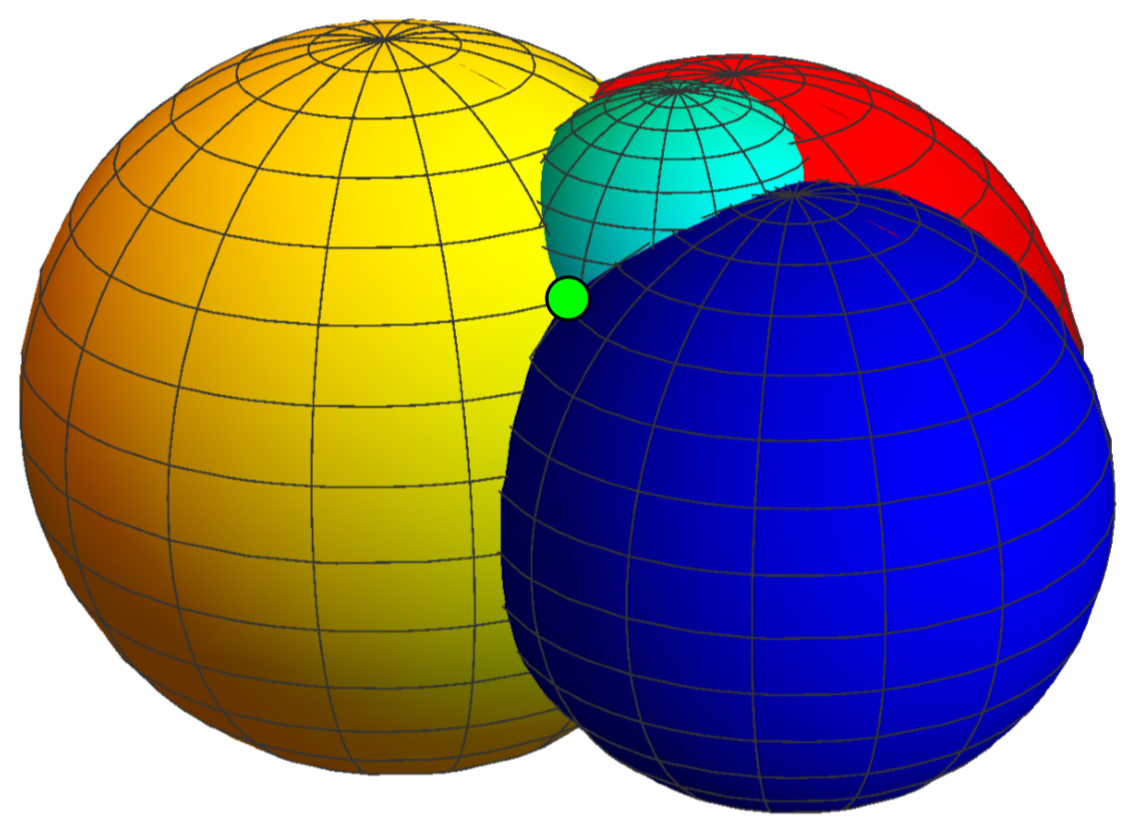
\includegraphics[width=0.95\linewidth]{quatroesferas.png}
				\end{minipage}
				\begin{minipage}{0.2\linewidth}
					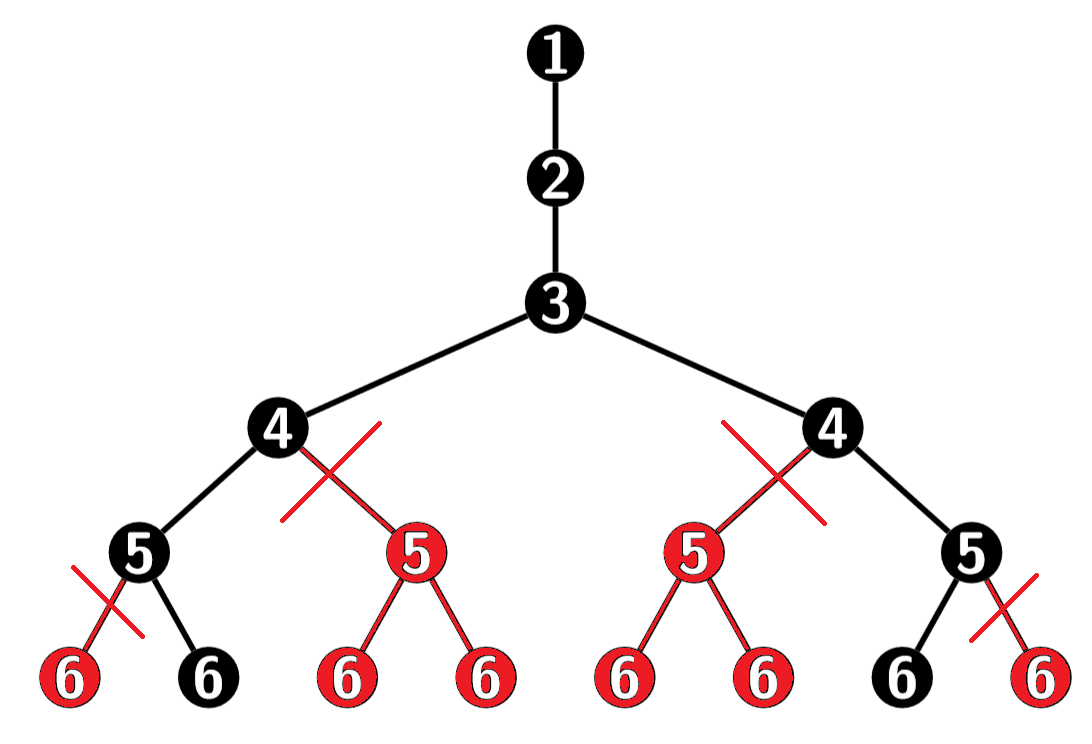
\includegraphics[width=1.5\linewidth]{prune.png}
				\end{minipage}
				\begin{minipage}{0.08\linewidth}
					\hspace{0.2cm}
				\end{minipage}
			\end{center}
		}	
	\end{frame}

	\begin{frame}
		\frametitle{\normalsize Algoritmo Branch-\&-Prune (BP)} 
		{
			\small
			Considerando $\mathbf x_{i} \in\mathbb{R}^3,i= 1, ...,n $ da forma $(x_{i1},x_{i2},x_{i3})$, temos:
			$$
			\begin{bmatrix}
				x_{i1}\\ 
				x_{i2}\\ 
				x_{i3}\\ 
				1
			\end{bmatrix}
			= B_{1}B_{2}\cdots B_{i}\begin{bmatrix}
				0\\ 
				0\\ 
				0\\ 
				1
			\end{bmatrix},
			$$
			$$
			B_1\: =\:
			\begin{bmatrix}
				1 & 0 & 0 & 0\\ 
				0 & 1 & 0 & 0\\ 
				0 & 0 & 1 & 0\\ 
				0 & 0 & 0 & 1
			\end{bmatrix},\:\:\:
			\: B_2\: =\:
			\begin{bmatrix}
				-1 & 0 & 0 & -d_{1,2}\\
				0 & 1 & 0 & 0\\ 
				0 & 0 & -1 & 0\\ 
				0 & 0 & 0 & 1
			\end{bmatrix},
			$$
			$$
			B_3\:=\:
			\begin{bmatrix}
				-\cos\theta_{1,3} & -\mbox{sen}\theta_{1,3} & 0 & -d_{2,3}\cos\theta_{1,3}\\ 
				\mbox{sen}\theta_{1,3} & -\cos\theta_{1,3} & 0 & d_{2,3}\mbox{sen}\theta_{1,3}\\ 
				0 & 0 & 1 & 0\\ 
				0 & 0 & 0 & 1
			\end{bmatrix},
			$$
			$$
			B_i\:=\:
			\begin{bmatrix}
				-c_{\theta_{i}} & -s_{\theta_{i}} & 0 & -d_{i-1,i}c_{\theta_{i}}\\ 
				s_{\theta_{i}}c_{\omega_{i}} & -c_{\theta_{i}}c_{\omega_{i}}
				& -s_{\omega_{i}} & d_{i-1,i}s_{\theta_{i}}c_{\omega_{i}}\\ 
				s_{\theta_{i}}s_{\omega_{i}} & -c_{\theta_{i}}s_{\omega_{i}} & c_{\omega_{i}} & d_{i-1,i}s_{\theta_{i}}s_{\omega_{i}}\\ 
				0 & 0 & 0 & 1
			\end{bmatrix}
			$$
			dado $s_{\theta_{i}}=\mbox{sen} (\theta_{i-2, i}),\: c_{\theta_{i}}=\cos (\theta_{i-2, i}),\: s_{\omega_{i}}=\mbox{sen} (\omega_{i-3, i}),\: c_{\omega_{i}}=\cos (\omega_{i-3, i})$.
		}	
	\end{frame}

	\section{Objetivo}
	
	\begin{frame}
		\frametitle{\normalsize Objetivo} 
		{
			\normalsize
			
			\begin{center}
				Queremos reescrever o BP usando a álgebra de quatérnios.
			\end{center}
		}	
	\end{frame}
	
	\section{BP com Quatérnios}
	
	\begin{frame}
		\frametitle{\normalsize Inicialização \cite{thompsonBi}} 
		{
			\begin{center}
				$x_1 = (0,0,0)$
				\\
				
				\vspace{0.5cm}
				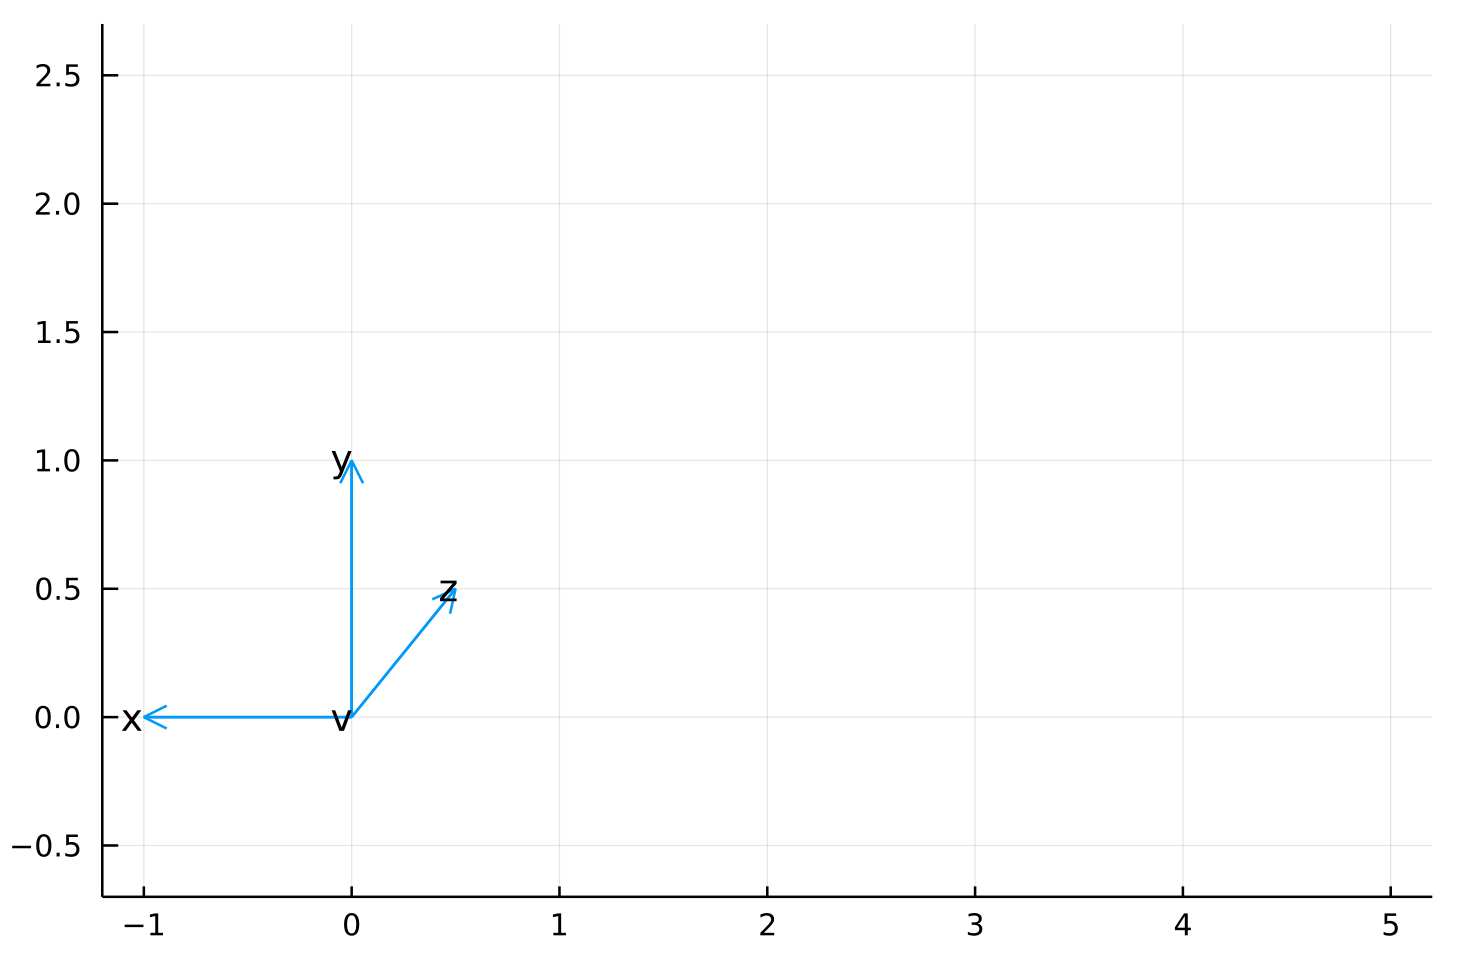
\includegraphics[width=0.8\linewidth]{1.png}
			\end{center}
		}	
	\end{frame}

	\begin{frame}
		\frametitle{\normalsize Inicialização} 
		{
			\begin{center}
				$x_2 = (\mathbf j)x_1(\mathbf j)^*$
				\\
				
				\vspace{0.5cm}
				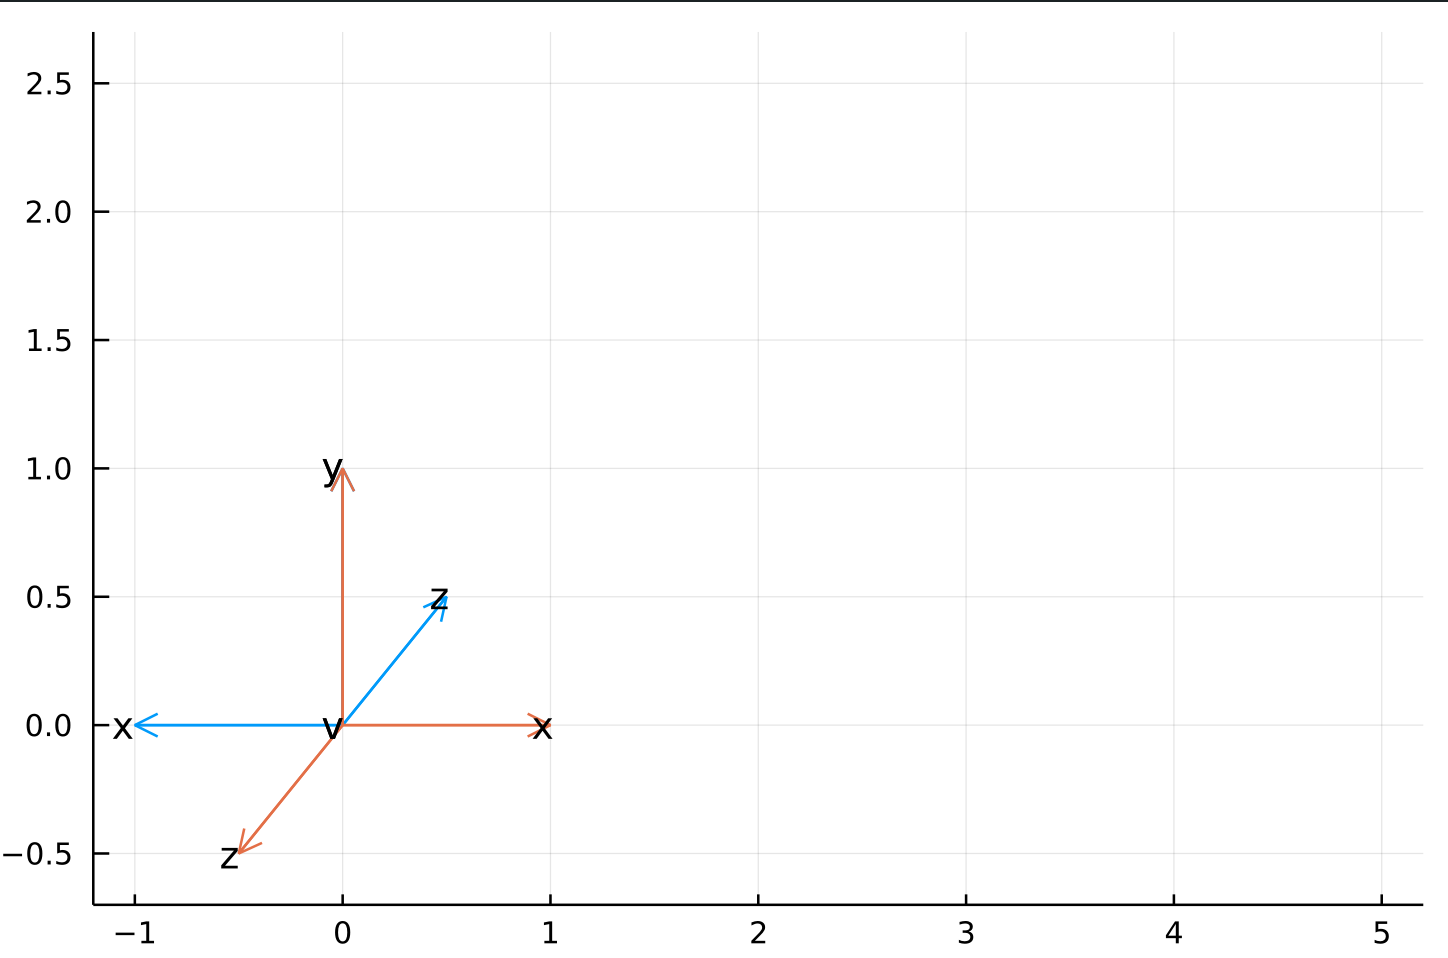
\includegraphics[width=0.8\linewidth]{2.png}
			\end{center}
		}	
	\end{frame}

	\begin{frame}
		\frametitle{\normalsize Inicialização} 
		{
			\begin{center}
				$x_2 = (\mathbf j)(x_1 + d_{1,2}\mathbf i)(\mathbf j)^*$
				\\
				
				\vspace{0.5cm}
				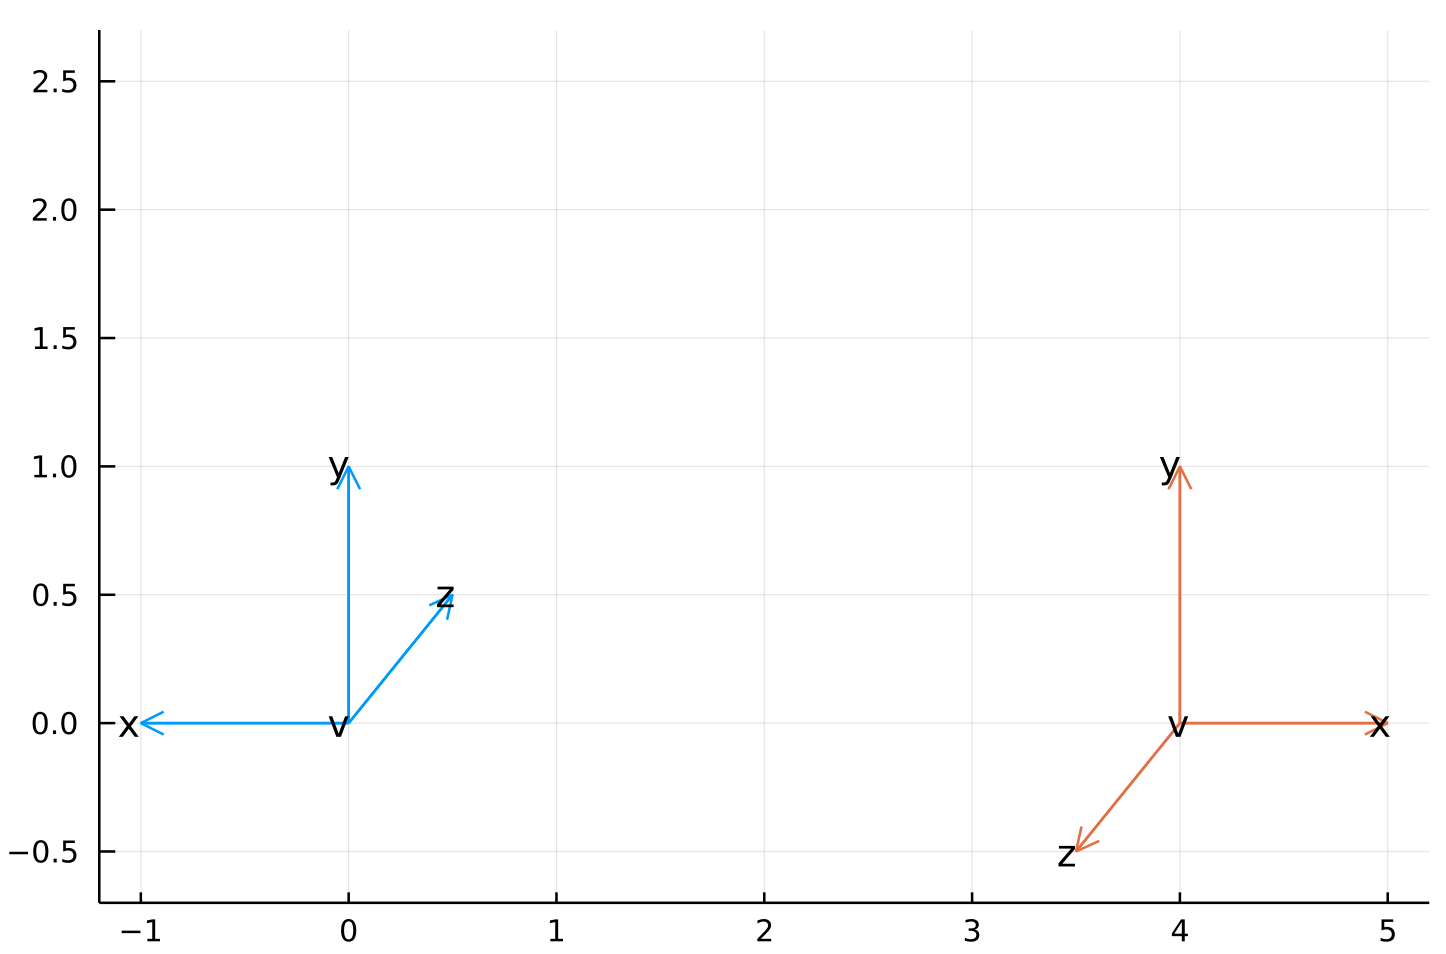
\includegraphics[width=0.8\linewidth]{3.png}
			\end{center}
		}	
	\end{frame}

	\begin{frame}
		\frametitle{\normalsize Inicialização} 
		{
			\begin{center}
				$x_3 = (\sin(\frac \theta 2) + \cos(\frac \theta 2)\mathbf k)(x_2)(\sin(\frac \theta 2) + \cos(\frac \theta 2)\mathbf k)^*$
				\\
				
				\vspace{0.5cm}
				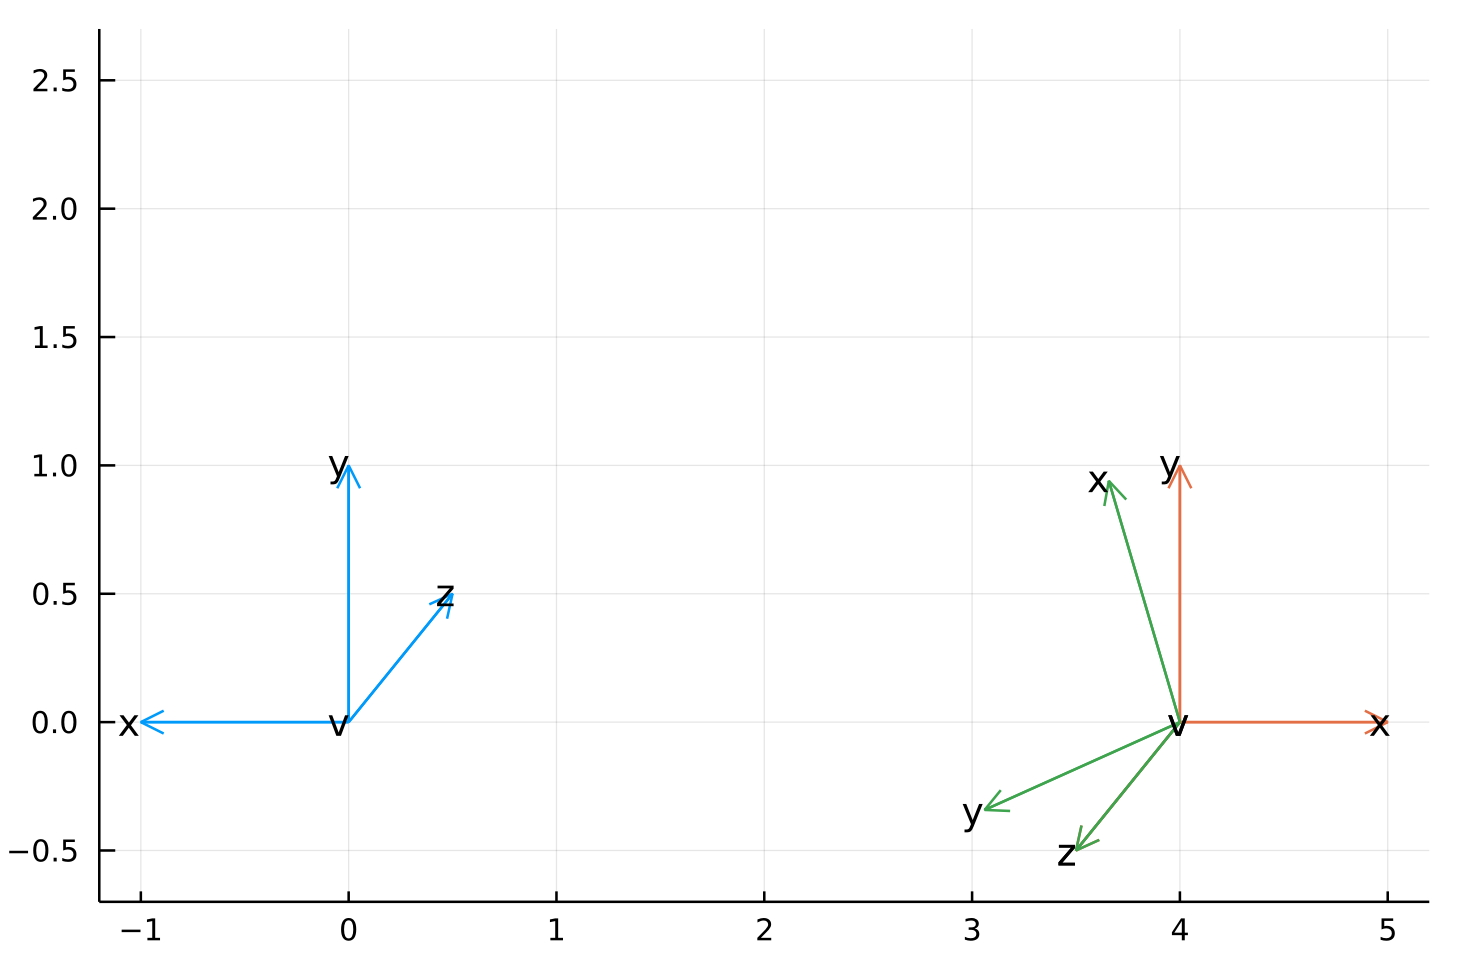
\includegraphics[width=0.8\linewidth]{4.png}
			\end{center}
		}	
	\end{frame}

	\begin{frame}
		\frametitle{\normalsize Inicialização} 
		{
			\begin{center}
				$x_3 = (\sin(\frac \theta 2) + \cos(\frac \theta 2)\mathbf k)(x_2 + d_{2,3}\mathbf i)(\sin(\frac \theta 2) + \cos(\frac \theta 2)\mathbf k)^*$
				\\
				
				\vspace{0.5cm}
				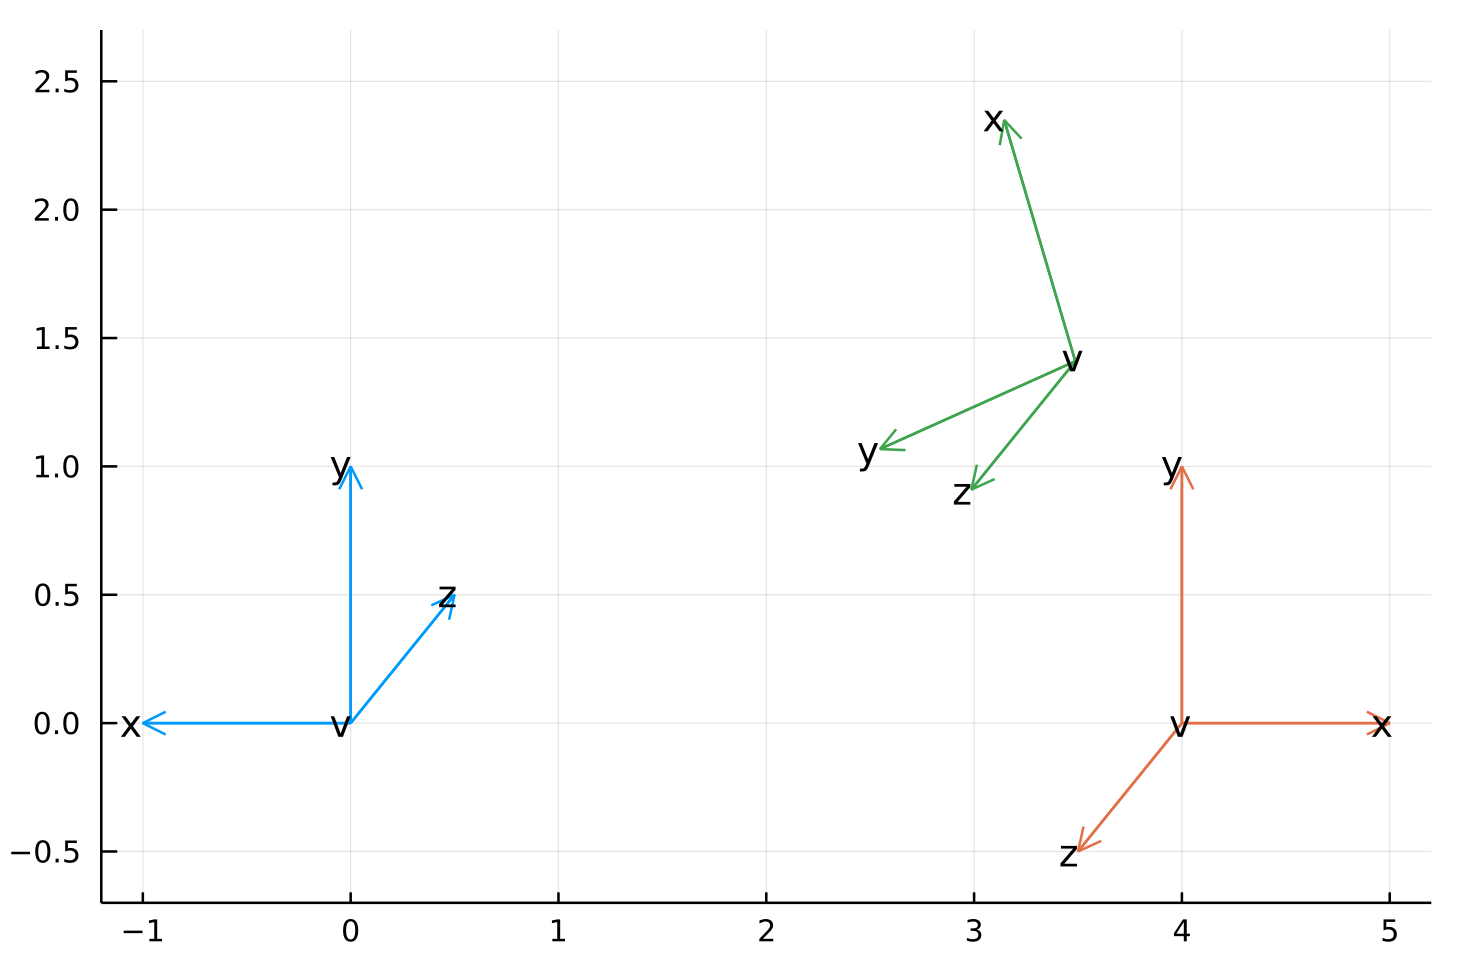
\includegraphics[width=0.8\linewidth]{5.png}
			\end{center}
		}	
	\end{frame}
	
	\begin{frame}
		\frametitle{\normalsize Branch} 
		{
			\begin{center}
				Ângulo diedral (ou, de torção)
				
				\vspace{0.5cm}
				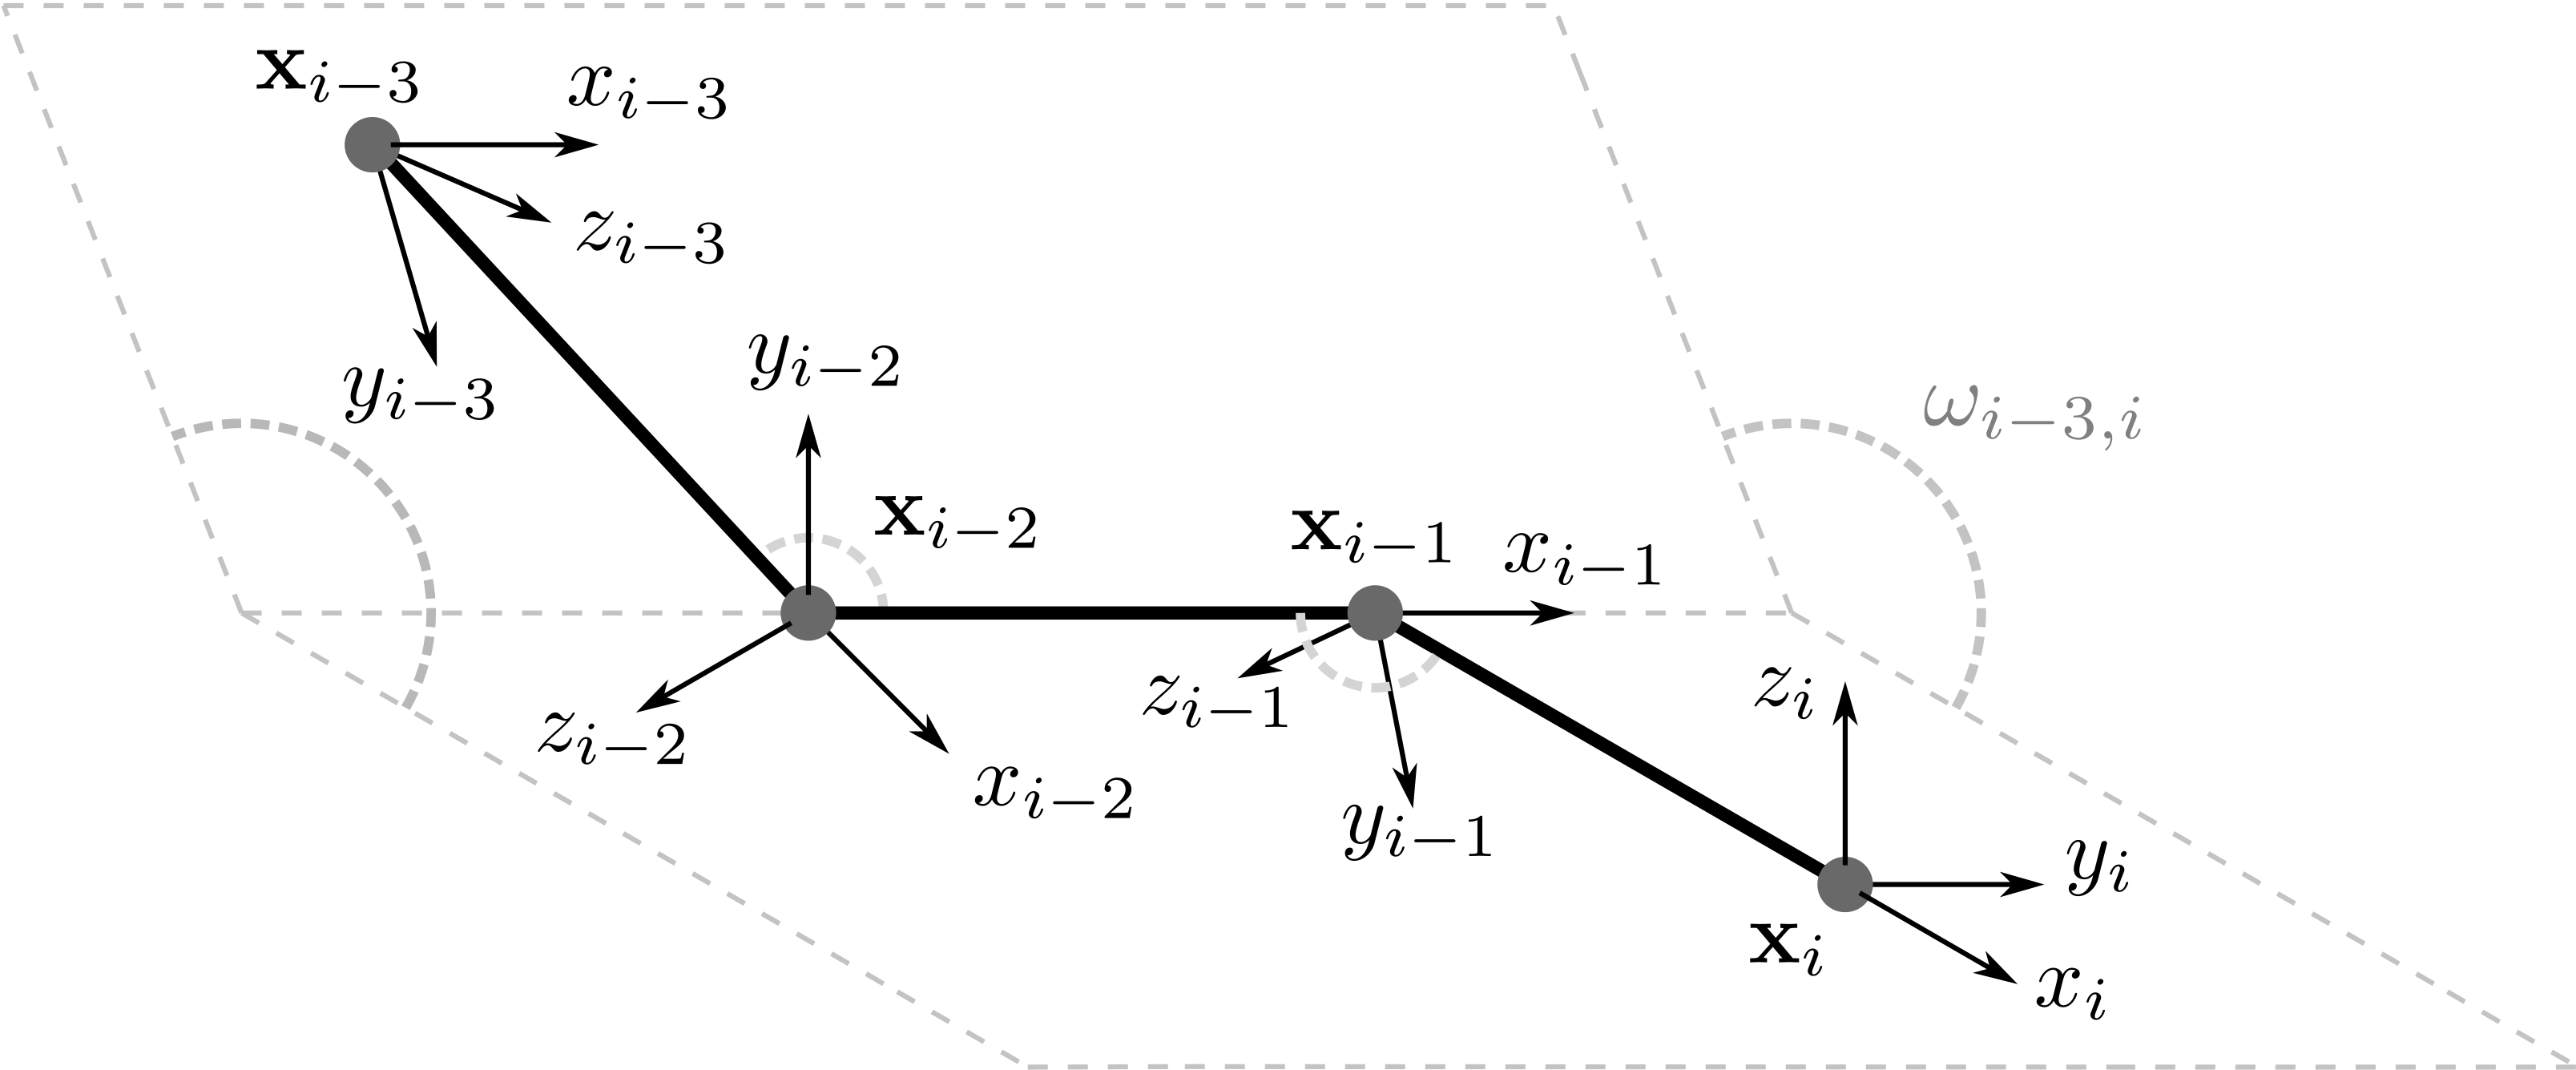
\includegraphics[width=0.8\linewidth]{genericConf-4Fidalgo.png}
				\vspace{0.2cm}			
				
				$\sin(\omega_{i-3,i}) = \sqrt{1-\cos^2(\omega_{i-3,i})}$
			\end{center}
		}	
	\end{frame}


	\begin{frame}
		\frametitle{\normalsize Branch} 
		{
			\begin{center}
				Fazendo $q_{i,\mathbf i} =  \cos(\frac {\omega_{i-3, i}} 2) + \sin(\frac {\omega_{i-3, i}} 2) \mathbf i$, temos que\\
				\vspace{0.2cm}
				$x_i^1 = (q_{i,\mathbf i})(x_{i-1})(q_{i,\mathbf i})^*$
				\\
				
				\vspace{0.5cm}
				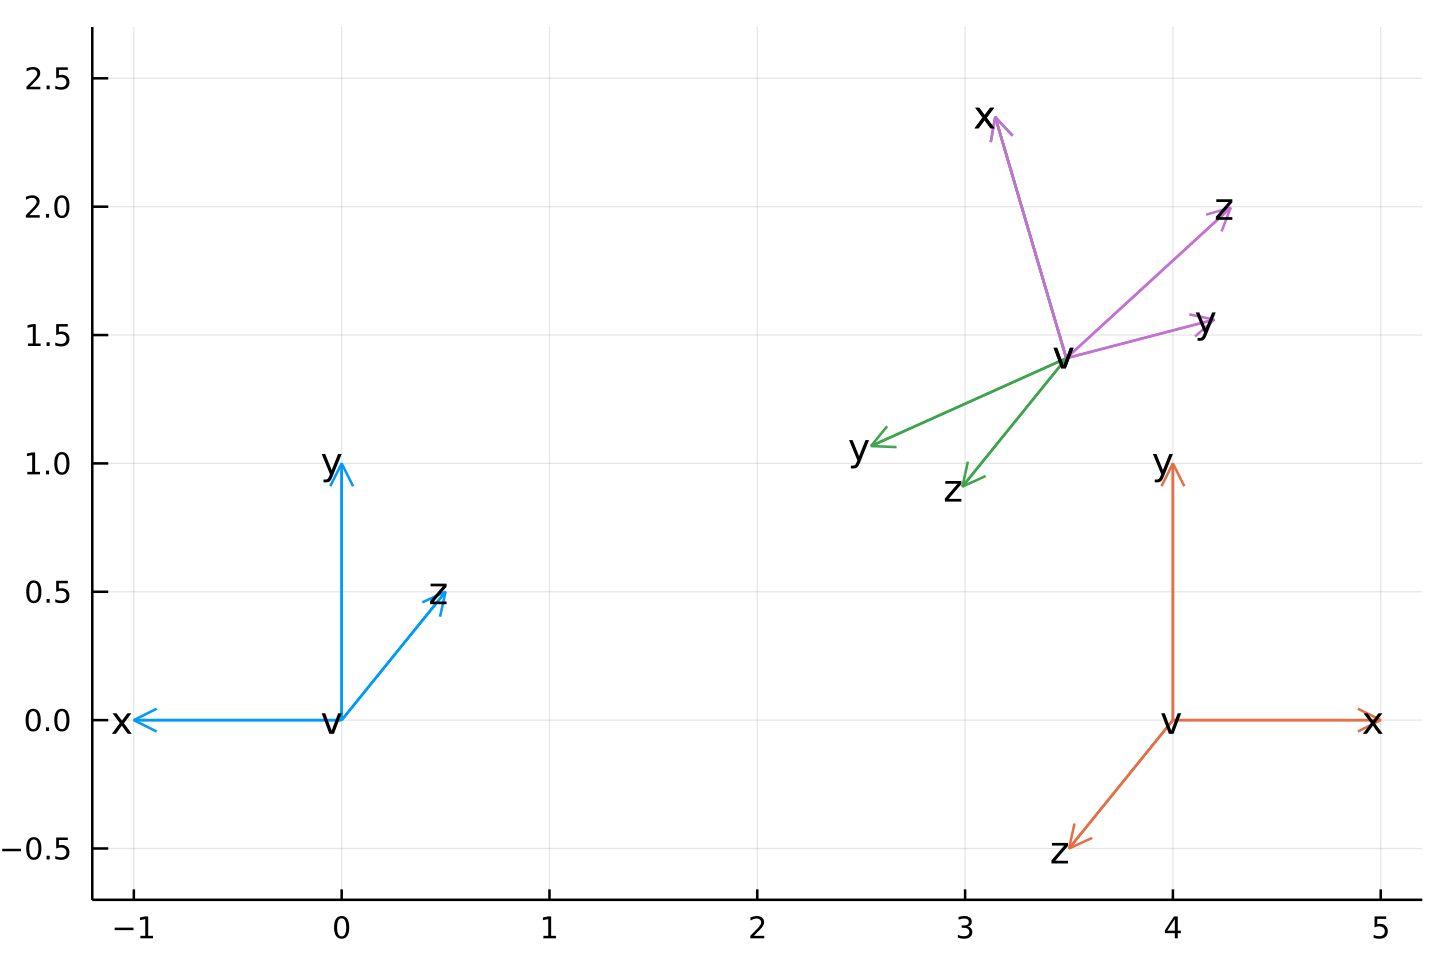
\includegraphics[width=0.8\linewidth]{6.png}
			\end{center}
		}	
	\end{frame}

	\begin{frame}
		\frametitle{\normalsize Branch} 
		{
			\begin{center}
				Ou, fazendo  $\cos(-\frac {\omega_{i-3, i}} 2) + \sin(-\frac {\omega_{i-3, i}} 2) \mathbf i = q_{i,\mathbf i}^*$, temos que\\
				\vspace{0.2cm}
				$x_i^0 = (q_{i,\mathbf i})^*(x_{i-1})(q_{i,\mathbf i})$
				\\
				
				\vspace{0.5cm}
				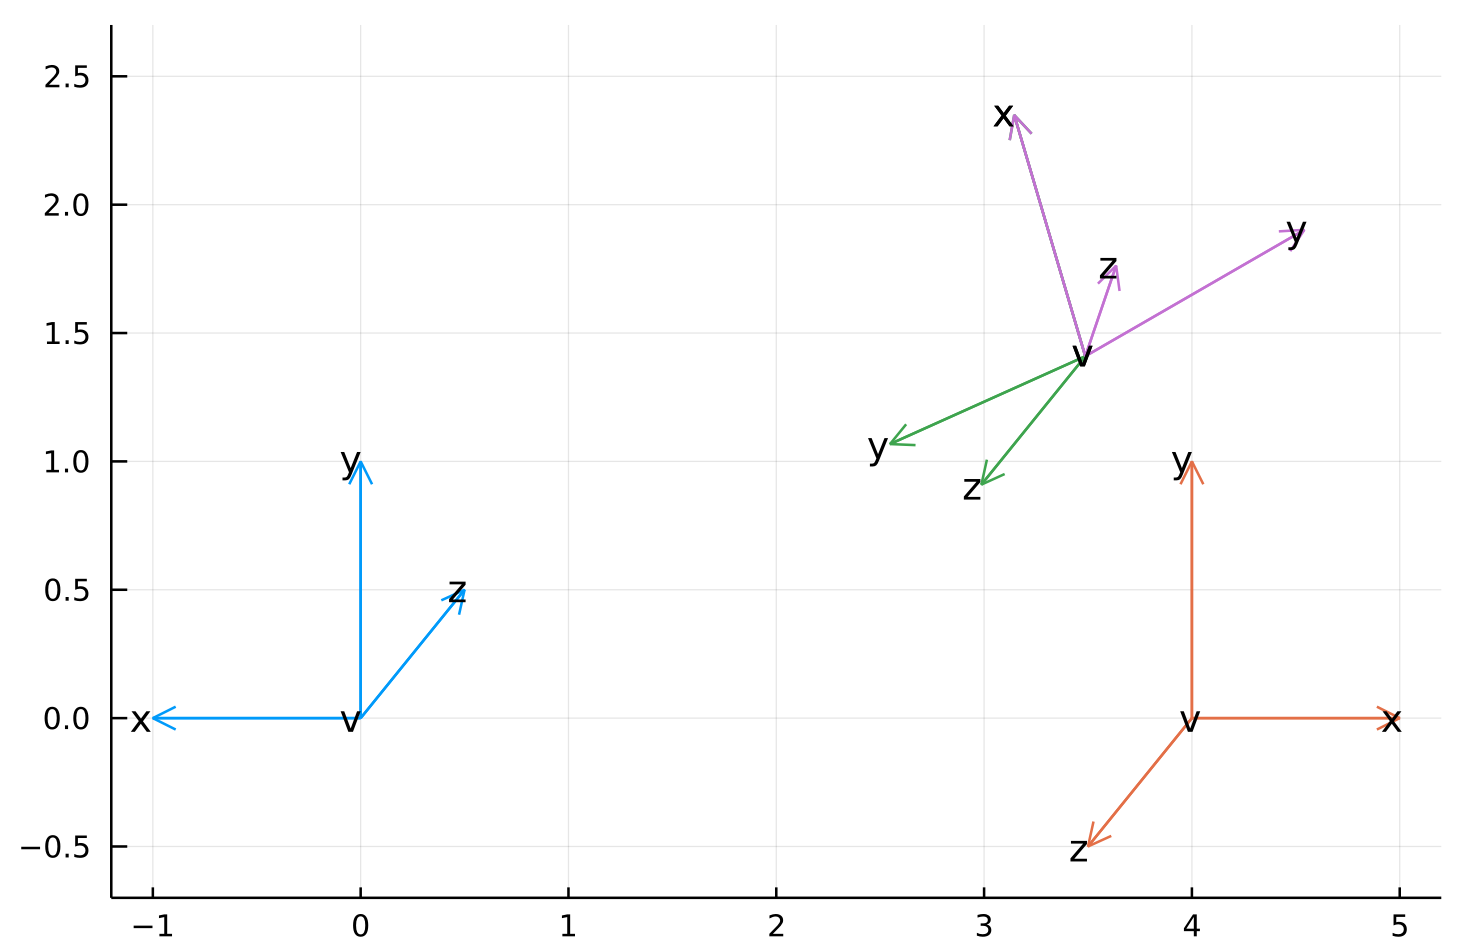
\includegraphics[width=0.8\linewidth]{6n.png}
			\end{center}
		}	
	\end{frame}

	\begin{frame}
		\frametitle{\normalsize Branch} 
		{
			\begin{center}
				E fazendo $q_{i, \mathbf k} = \sin(\frac {\theta_{i-2, i}} 2) + \cos(\frac {\theta_{i-2, i}} 2)\mathbf k$, temos que\\
				\vspace{0.2cm}
				$x_i^1 = (q_{i,\mathbf i})(q_{i, \mathbf k})(x_{i-1})(q_{i, \mathbf k})^*(q_{i,\mathbf i})^*$
				\\
				
				\vspace{0.5cm}
				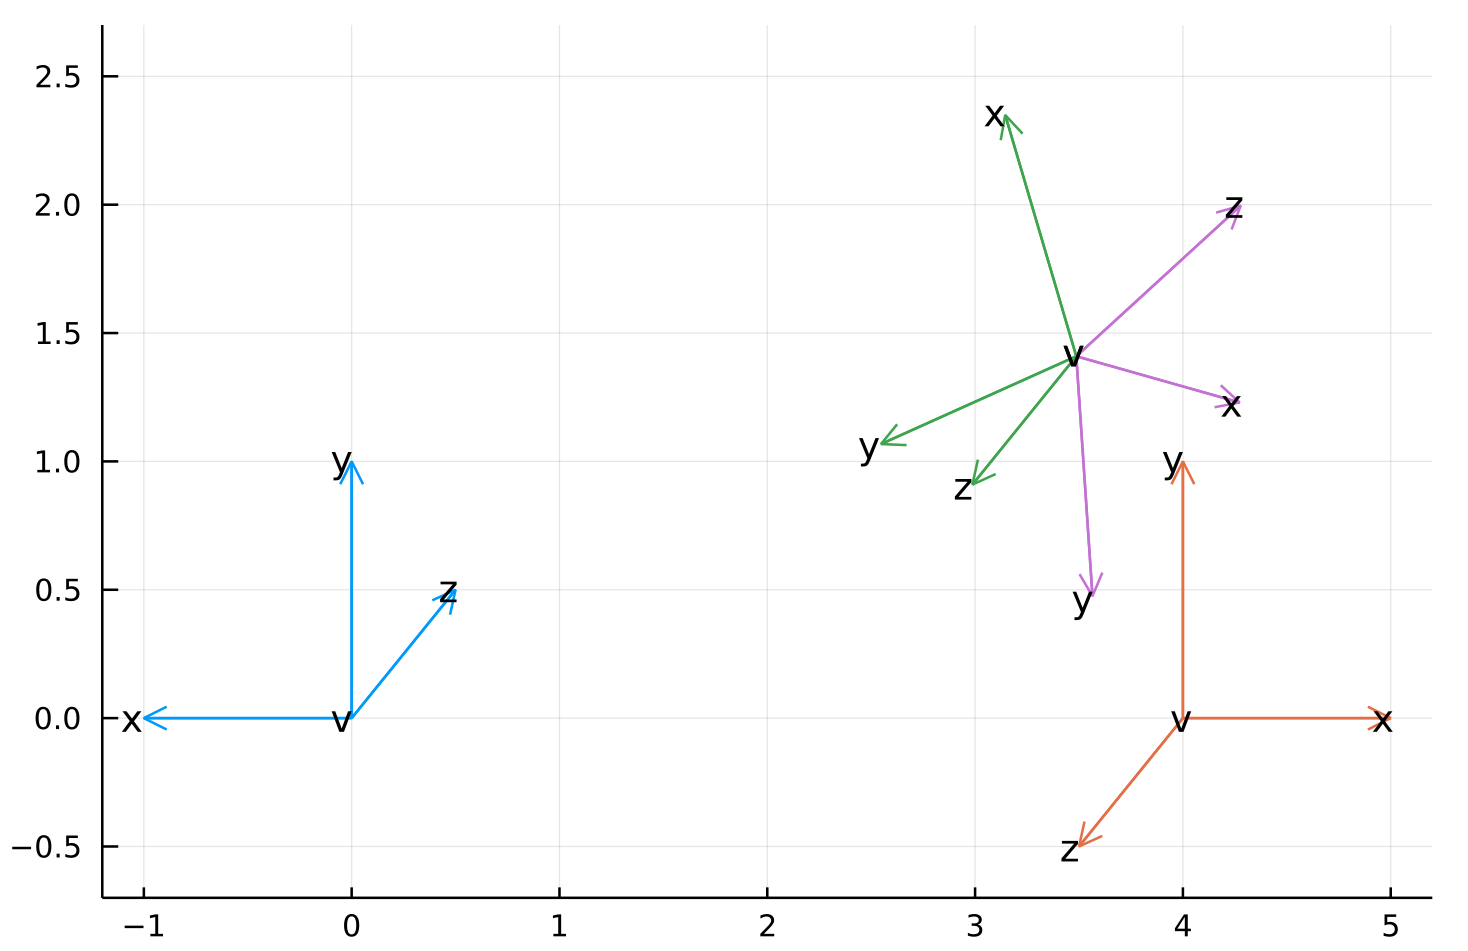
\includegraphics[width=0.8\linewidth]{7.png}
			\end{center}
		}	
	\end{frame}

	\begin{frame}
		\frametitle{\normalsize Branch} 
		{
			\begin{center}
				\vspace{0.5cm}
				$x_i^1 = (q_{i,\mathbf i})(q_{i, \mathbf k})(x_{i-1} + d_{i,i-1}\mathbf i)(q_{i, \mathbf k})^*(q_{i,\mathbf i})^*$
				\\
				
				\vspace{0.5cm}
				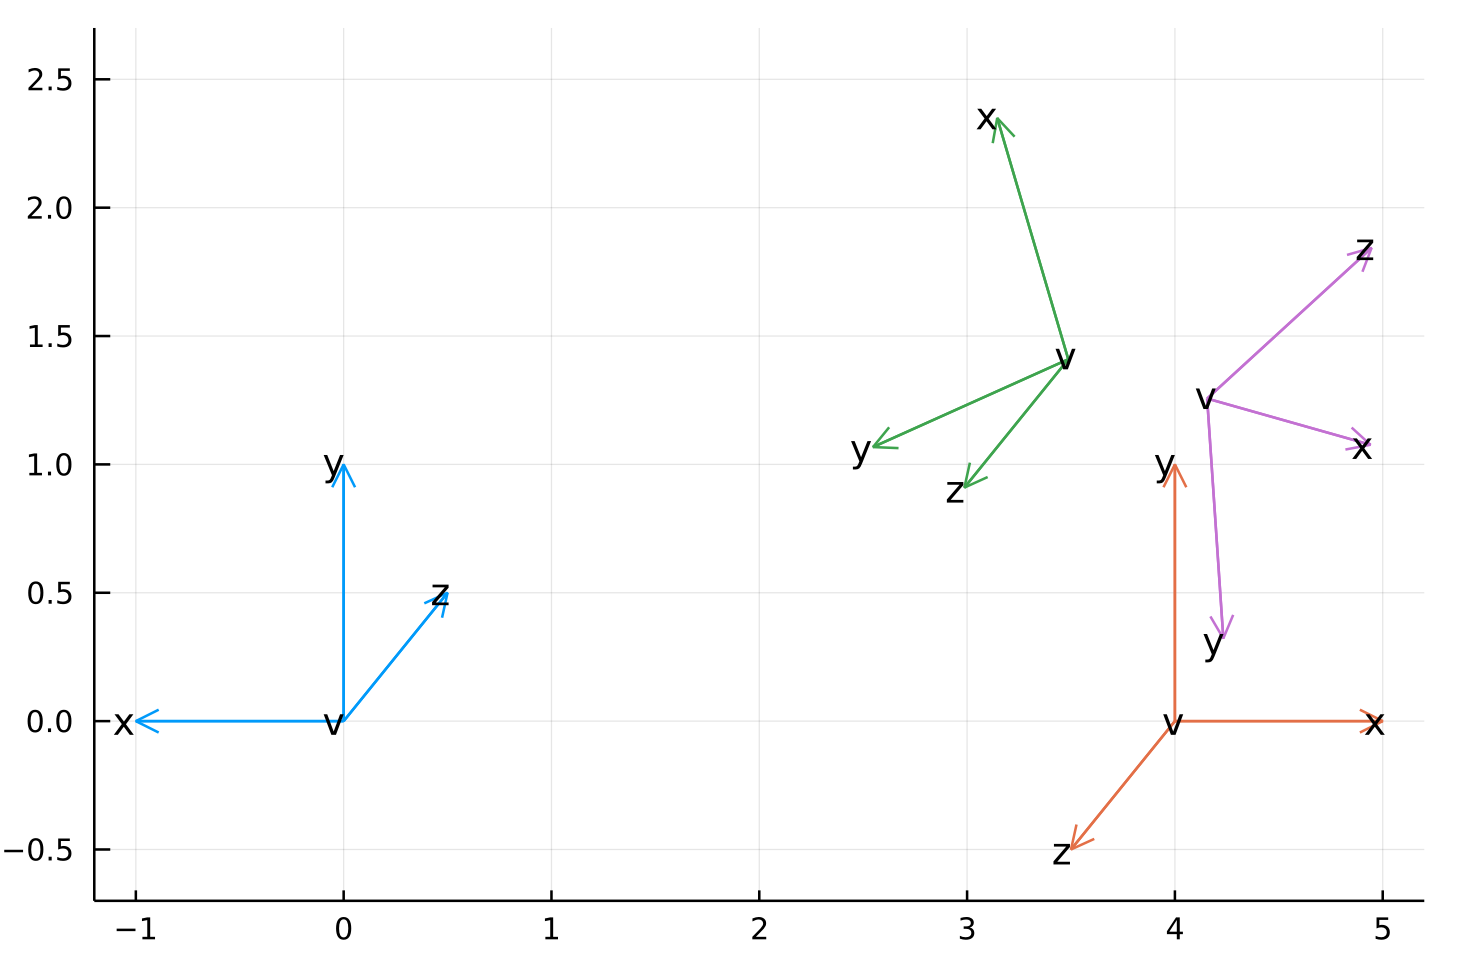
\includegraphics[width=0.8\linewidth]{8.png}
			\end{center}
		}	
	\end{frame}
	
	\begin{frame}
		\frametitle{\normalsize Calculo iterativo} 
		{
			
			Perceba que, se chamarmos $q_1 = 1, q_2 = -\mathbf j$, podemos reescrever o quatérnio $x_2$ como $$x_2 = \mathbf j(x_1+d_{1,2}\mathbf i)(-\mathbf j) = q_1(q_2(\mathbf 0 + d_{1,2}\mathbf i)q_2^* + \mathbf 0)q_1^* \ =\  q_1q_2(\mathbf 0 + d_{1,2})\mathbf iq_1^*q_2^* + q_1\mathbf 0q_1^*,$$ e se chamarmos $\mathbf t_2 = 0+d_{1,2}\mathbf i$ e $\mathbf 0 = \mathbf t_1$ para identificar as translações envolvendo, respectivamente, a $x_1$ e a $x_2$, temos $$x_2 = q_1q_2\mathbf t_2q_2^*q_1^* + q_1\mathbf t_1q_1^* \ = \ (q_1q_2)\mathbf t_2 (q_1q_2)^* + x_1.$$
			
			\begin{center}
				Se renomearmos os quatérnios de rotação e rearranjarmos os termos, 
				$$
				\begin{tabular}{rcl}
					$\mathbf x_1 $& $= $ & $q_1(\mathbf \mathbf t_1)q_1^*$\\
					$\mathbf x_2 $& $= $ & $(q_1q_2)\mathbf t_2 (q_1q_2)^* + \mathbf x_1$\\
					$\mathbf x_3 $& $= $ & $(q_1q_2q_3)\mathbf t_3(q_1q_2q_3)^* + \mathbf x_2$	
				\end{tabular}
				$$
				e, para $i\geq 4$,
				$$\mathbf x_i = q_1(q_2(q_3(\cdots q_i(\mathbf t_i)q_i^*\cdots+\mathbf t_3)q_3^*+ \mathbf t_2)q_2^*+ \mathbf t_1)q_1^* \ = $$ $$= \ (q_1q_2\dots q_i)\mathbf t_i(q_1q_2\dots q_i)^* + \mathbf x_{i-1}.$$
			\end{center}
		}	
	\end{frame}
	
	\begin{frame}
		\frametitle{\normalsize Prune} 
		{
			\begin{center}
				Assim,
				$$
				\begin{tabular}{rll}
					$\mathbf x_i^0 =$&  $(q_1q_2\dots q_i^*)\mathbf t_i(q_1q_2\dots q_i^*)^*$& $+ \mathbf x_{i-1}$\\
					$\mathbf x_i^1 =$& $(q_1q_2\dots q_i)\mathbf t_i(q_1q_2\dots q_i)^*$& $+ \mathbf x_{i-1}$
				\end{tabular}.
				$$
				\\	
				\vspace{2cm}
				
				Não há modificações no passo de prune.
			\end{center}
		}	
	\end{frame}
	
	\section{Simulações computacionais}
	
	\begin{frame}
		\frametitle{\normalsize Ambiente desenvolvido} 
		{
			\small
			
			
			\begin{itemize}
				\item HCProt\footnote{https://github.com/caomem/PDBReader}: Software para preprocessamento de instâncias PDB, chamado HCProt. Vesão com ferramentas visuais para facilitar a criação de ordenações manuais.
				\begin{center}
					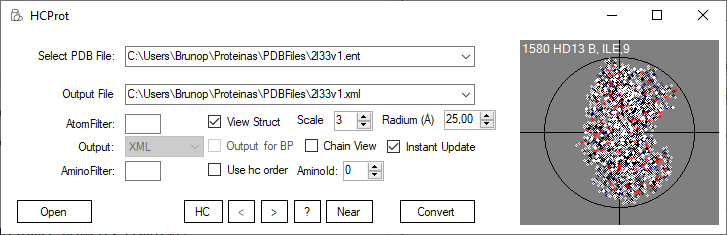
\includegraphics[width=0.8\linewidth]{molproj.png}	
				\end{center}
				\item HCProtCLI\footnote{https://github.com/caomem/HCProtCLI}: interface linha de comando para a automação do preprocessamento;
				\vspace{0.2cm}
				\item MolecularConformation.jl\footnote{https://github.com/evcastelani/MolecularConformation.jl}: Pacote Julia do algoritmo BP, desenvolvido em colaboração com Emerson Vitor Castelani.
			\end{itemize}
		}	
	\end{frame}

	\begin{frame}
		\frametitle{\normalsize Resultados computacionais} 
		{			
			\begin{table}[H]
				\centering
				{\footnotesize
					\begin{tabular}{||rS[table-format=1.3e+2]S[table-format=1.4e+2]S[table-format=1.4e+2]||}
						\hline
						\multicolumn{1}{||c}{Problema} & \multicolumn{1}{c}{LDE} & \multicolumn{1}{c}{RMSD} & \multicolumn{1}{c||}{Tempo} \\
						\hline
						pdb1ba5 & 4.257e-21 & 1.8249e-10 & 1.5480e-01 \\
						pdb1d1n & 4.268e-11 & 1.1200e-11 & 4.3957e-01 \\
						pdb1dp3 & 2.048e-10 & 8.2794e-11 & 3.4111e-01 \\
						pdb1du1 & 2.921e-21 & 1.1862e-12 & 2.2095e-02 \\
						pdb1fcl & 1.650e-10 & 2.5527e-12 & 5.0979e-01 \\
						pdb1fd6 & 3.248e-20 & 1.4000e-11 & 2.9719e-01 \\
						pdb1i2u & 4.779e-22 & 9.1058e-12 & 9.5673e-02 \\
						pdb1i2v & 3.179e-22 & 9.5660e-13 & 1.3251e-01 \\
						pdb1jlz & 3.852e-22 & 8.6556e-12 & 2.9969e-02 \\
						pdb1k0v & 8.541e-23 & 3.0991e-13 & 2.3770e-01 \\ \hline
					\end{tabular}}
					\caption{Simulações computacionais sobre o algoritmo \texttt{QuaternionBP} em exemplares reais.}\label{table:improvreal}
				\end{table}
		}	
	\end{frame}
	
	\section{Referências}
	%Slide refe
	\begin{frame}		
		
		{\footnotesize
		\bibliographystyle{unsrt}
		\bibliography{references}}
	\end{frame}
	
	%Slide End
	\begin{frame}
		\begin{center}
			\vspace{1.5cm}
			Obrigado!\\
			\hspace{-4.5cm}
			
\includegraphics[scale=0.2]{logo.png}
			
			\vspace{-2.7cm}
			\hspace{5.5cm}
			
\includegraphics[scale=0.038]{logo_ufsc.png}
			
			\vspace{0.5cm}
			Contato: g.philippi@grad.ufsc.br\\ UFSC - Blumenau
		\end{center}
	\end{frame}
	
\end{document}